\documentclass{beamer}
\usepackage{
    graphicx, float, caption,
    amsmath, longtable, booktabs,
    textpos, blindtext, scrextend,
    apacite
}
\usepackage[flushleft]{threeparttable}
\usepackage[font=small, labelfont=bf]{subcaption}

%% MARK: Beamer Setup
\usetheme{Darmstadt}
% Remove the useless and unsightly black bar at the top of the slides
\setbeamertemplate{headline}{}
% Remove the navigation thing at the bottom of the slides.
\setbeamertemplate{navigation symbols}{}
% Colors for Auburn University from their marketing materials
% http://www.ocm.auburn.edu/graphicservices/colors.html
\definecolor{auburn_orange}{RGB}{232, 119, 34}
\definecolor{auburn_blue}{RGB}{12, 35, 64}
% Set the color of the slide headers to auburn blue
\setbeamercolor{structure}{fg=auburn_blue}

%% MARK: Frontmatter
\title{Playing Super Mario Bros. with Deep Reinforcement Learning}
\author{Christian Kauten, Chaowei Zhang}
\institute{Auburn University}
\date{April 23, 2018}

%% MARK: Slides
\begin{document}
% title slide
\frame{\titlepage}



\begin{frame}{Problem}
\begin{minipage}{\textwidth}
%
\begin{minipage}{0.5\textwidth}
\begin{itemize}
    \item{Atari 2600}
        \begin{itemize}
        \item{Breakout, Enduro, Pong, Seaquest, Space Invaders}
        \item{Stella}
        \end{itemize}
    \item{NES}
        \begin{itemize}
        \item{Super Mario Bros.}
        \item{FCEUX}
        \end{itemize}
\end{itemize}
\end{minipage}
%
\hfill
%
\begin{minipage}[t]{0.5\textwidth}
\centering
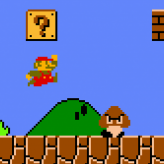
\includegraphics[width=0.75\textwidth]{img/smb} \\
$\Downarrow$ \\
$f : \mathcal{S} \to \mathcal{A}$ \\
$\Downarrow$ \\
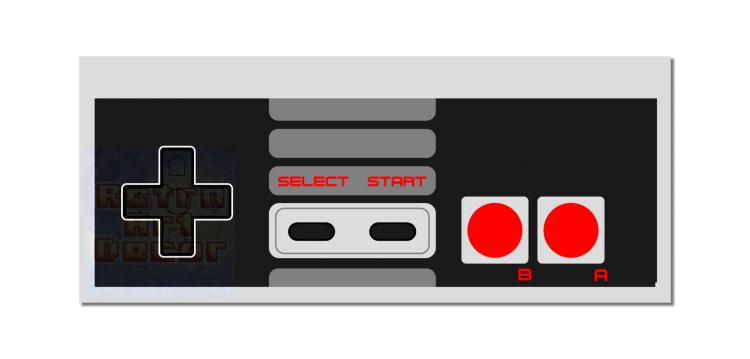
\includegraphics[width=0.85\textwidth]{img/nes}
\end{minipage}
%
\end{minipage}
\end{frame}



\begin{frame}{Dataset}
\begin{minipage}{\textwidth}
%
\begin{minipage}{0.35\textwidth}
\centering
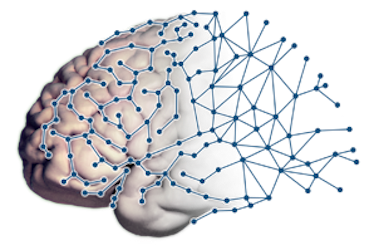
\includegraphics[width=\textwidth]{img/brain}
\end{minipage}
%
\hfill
%
\begin{minipage}{0.6\textwidth}
\begin{itemize}
    \item{Defined by the ROM for each game}
    \item{Experience Replay of $1000000$ experiences}
    \item{Generated using "bootstrapping"}
    \item{Networks train on random mini-batches of $32$ experiences every $4$ decisions}
\end{itemize}
\end{minipage}
%
\end{minipage}
\end{frame}



\begin{frame}{Methods}
\framesubtitle{Double Deep-Q Learning}

\begin{equation}
y = r + (1 - d) \gamma \max_{a' \in \mathcal{A}} Q(s', a', \theta_{target})
\end{equation}

\begin{equation}
\hat{y} = Q(s, a, \theta)
\end{equation}

\begin{equation}
L(\theta) =
\mathbb{E}_{(s, a, r, d, s') \sim U(D)} \bigg[ L_{\delta}(y, \hat{y}) \bigg]
\label{eqn:deep-q-alg}
\end{equation}

\begin{equation}
L_{\delta}(y, \hat{y}) = \begin{cases}
      \frac{1}{2} (y - \hat{y})^2                & |y - \hat{y}| \leq \delta \\
      \delta |y - \hat{y}| - \frac{1}{2}\delta^2 & \textbf{otherwise} \\
\end{cases}
\label{eqn:huber}
\end{equation}

\end{frame}



\begin{frame}{Methods}
\framesubtitle{Dueling Deep-Q Network}
\begin{figure}
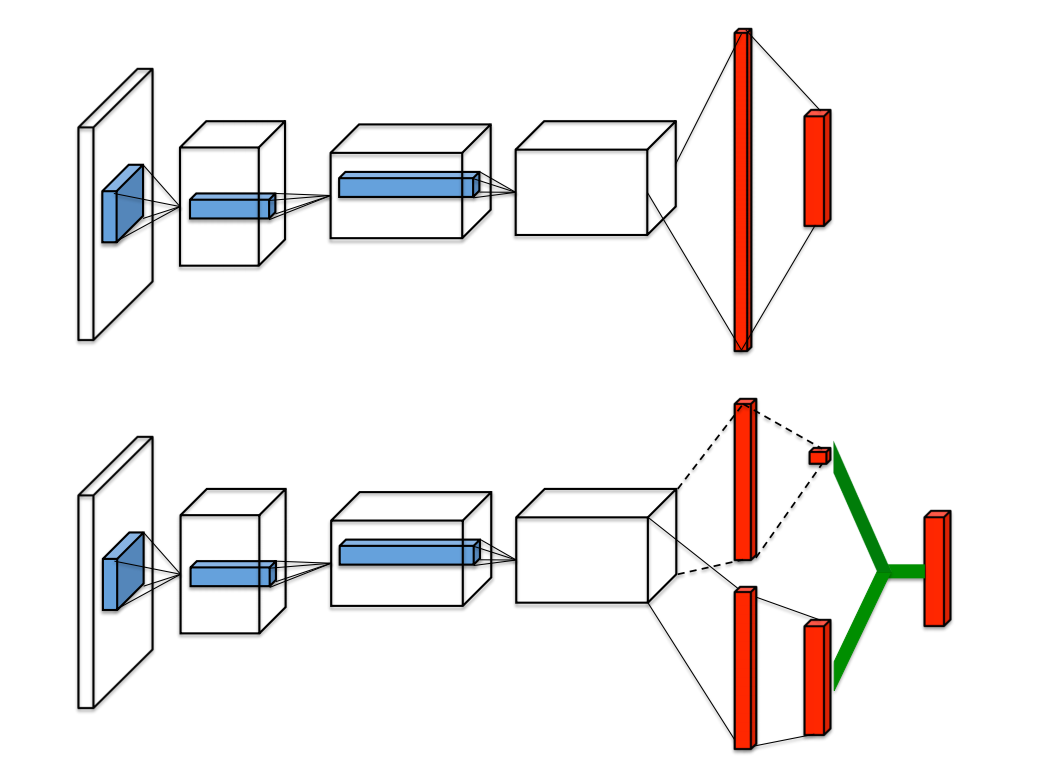
\includegraphics[width=0.9\textwidth]{img/dueling-deep-q}
\caption*{Deep-Q Network (top) and Dueling Deep-Q Network (Bottom)}
\end{figure}
\end{frame}



\begin{frame}{Results}
\framesubtitle{Atari}

\begin{minipage}[t]{\textwidth}
    \begin{minipage}{0.3\textwidth}
    \begin{figure}
    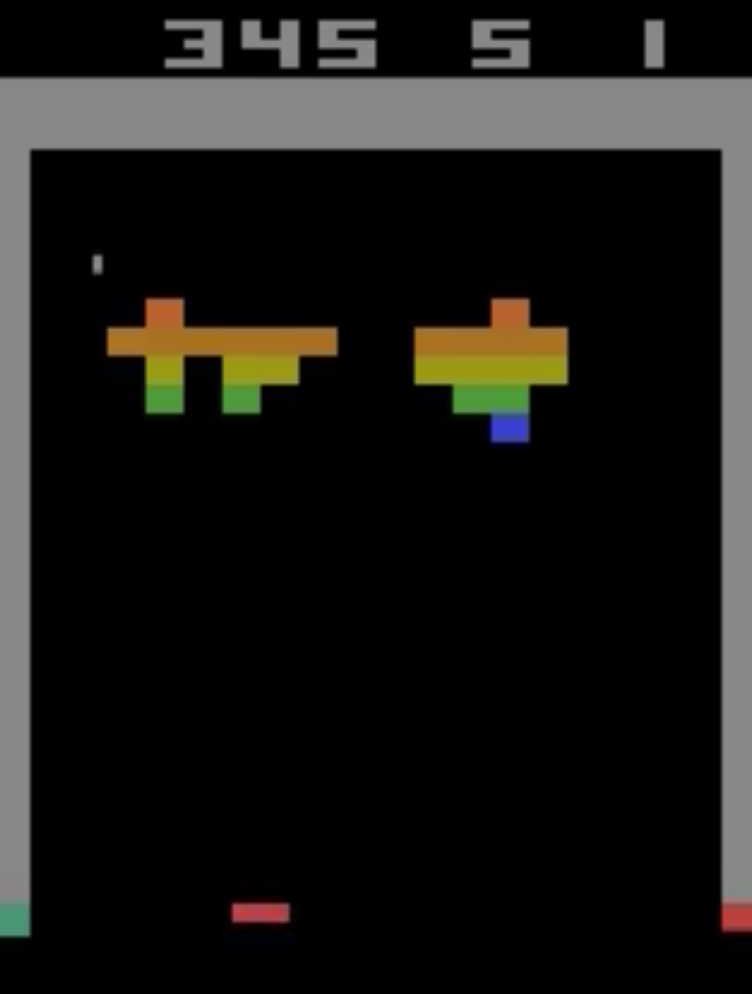
\includegraphics[height=0.35\textheight]{img/Breakout}
    \caption*{Breakout}
    \end{figure}
    \end{minipage}
    \hfill
    \begin{minipage}{0.3\textwidth}
    \begin{figure}
    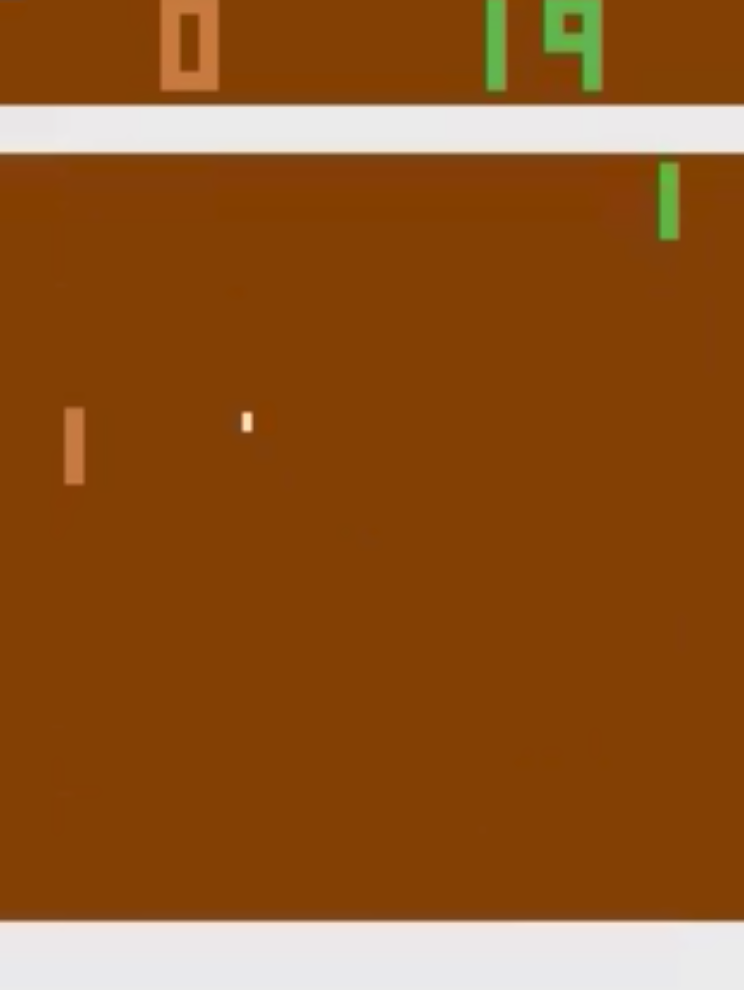
\includegraphics[height=0.35\textheight]{img/Pong}
    \caption*{Pong}
    \end{figure}
    \end{minipage}
    \hfill
    \begin{minipage}{0.3\textwidth}
    \begin{figure}
    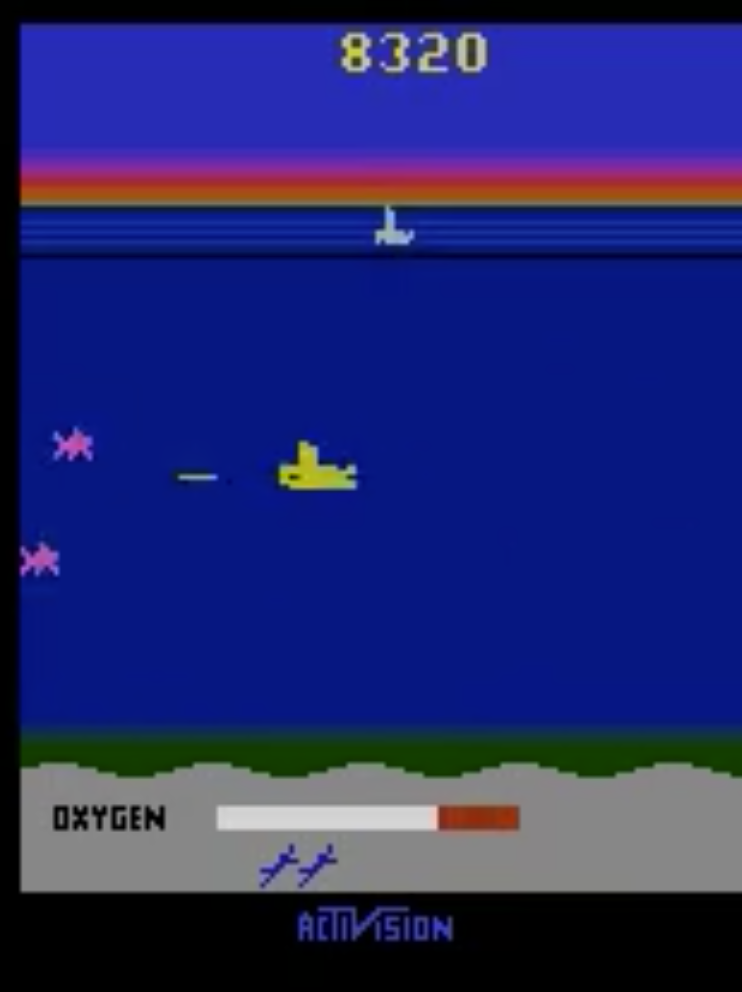
\includegraphics[height=0.35\textheight]{img/Seaquest}
    \caption*{Seaquest}
    \end{figure}
    \end{minipage}
\end{minipage}

\begin{minipage}[t]{\textwidth}
    \begin{table}
    \caption{Mean cumulative reward over $100$ validation episodes.}
    \begin{threeparttable}
        \begin{tabular}{||c c c c c c||}
        \hline
        & Breakout & Enduro & Pong & Seaquest & Space Invaders \\ [0.5ex]
        \hline\hline
        DDDQN & 363 & \textbf{330} & \textbf{19.7} & \textbf{8015} & 999 \\
        \hline
        DQN & \textbf{401} & 301 & 18.9 & 5286 & \textbf{1976} \\
        \hline
        Random & 1 & 0 & -21 & 103 & 138 \\
        \hline
        \end{tabular}
    \begin{tablenotes}
        \small
        \item $^*$ DDDQN trains for $1e7$ frames while DQN trains for $5e7$ frames.
    \end{tablenotes}
    \end{threeparttable}
    \end{table}
\end{minipage}

\end{frame}



\begin{frame}{Results}
\framesubtitle{Super Mario Bros}
\begin{minipage}{\textwidth}
%
\begin{minipage}{0.4\textwidth}
\begin{figure}
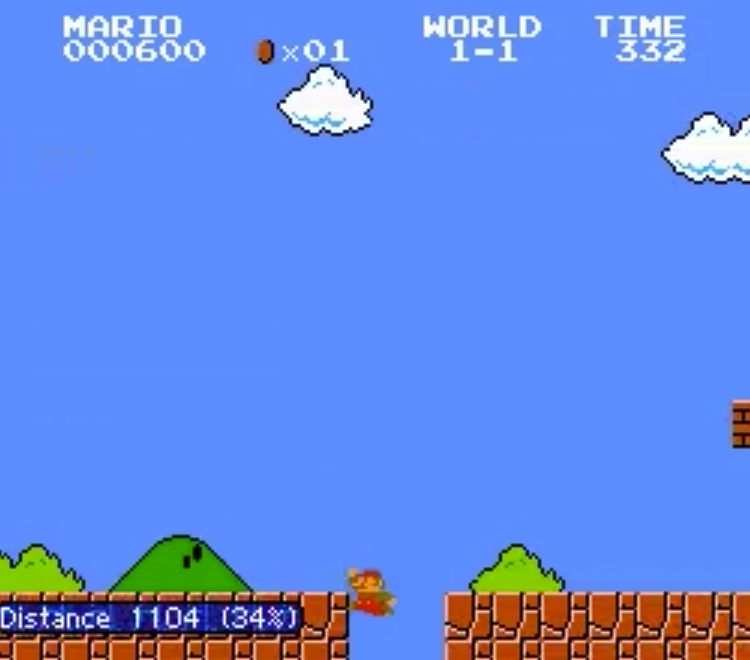
\includegraphics[width=\textwidth]{img/smb_clip}
\caption*{The agent struggles to detect holes in the ground and frequently
jumps into them.}
\end{figure}
\end{minipage}
%
\hfill
%
\begin{minipage}{0.5\textwidth}
    \begin{table}
    \centering
    \caption{Terminal $x$ position over $100$ validation episodes.}
    \begin{threeparttable}
    \begin{tabular}{||c c c c||}
    \hline
    & Min & Mean & Max \\ [0.5ex]
    \hline\hline
    DDDQN & \textbf{268} & \textbf{780} & \textbf{1436} \\
    \hline
    Random & 77 & 372 & 656 \\
    \hline
    \end{tabular}
    \begin{tablenotes}
        \small
        \item $^*$ DDDQN trains for $1e7$ frames.
    \end{tablenotes}
    \end{threeparttable}
    \end{table}
\end{minipage}
%
\end{minipage}
\end{frame}

\begin{frame}{Demo}
\begin{itemize}
\item{\href{https://youtu.be/6zf201DJrw0}{\textbf{Breakout}}}
\item{\href{https://youtu.be/6gAyvNIR-nk}{\textbf{Enduro}}}
\item{\href{https://youtu.be/MbYwTWhgMuE}{\textbf{Pong}}}
\item{\href{https://youtu.be/x12iHhEAOdg}{\textbf{Seaquest}}}
\item{\href{https://youtu.be/Zm6RGYQlTsU}{\textbf{Space Invaders}}}
\item{\href{https://youtu.be/H1Vmr5pm9B0}{\textbf{Super Mario Bros}}}
\end{itemize}
\end{frame}

\begin{frame}{Conclusions}
\begin{itemize}
    \item{DDDQN outperforms DQN in a fraction of the time in some cases}
    \item{DDDQN can play Mario with rudimentary confidence after $\approx 1e6$ experiences}
    \item{DDDQN generalizes across domains with no tweaking}
    \item{Engineering problems can have an immense impact on Deep-Learning work-flows}
    \item{Reward schemes get challenging to design in more complex environments}
\end{itemize}
\end{frame}

\begin{frame}{Q\&A}
\centering
Questions \& Answers
\end{frame}

\end{document}
